\documentclass[lettersize,journal]{IEEEtran}
\usepackage{amsmath,amsfonts}
\usepackage{algorithmic}
\usepackage{algorithm}
\usepackage{array}
\usepackage[caption=false,font=normalsize,labelfont=sf,textfont=sf]{subfig}
\usepackage{textcomp}
\usepackage{stfloats}
\usepackage{url}
\usepackage{verbatim}
\usepackage{graphicx}
\usepackage{cite}
\usepackage{BookTabs}
\usepackage{siunitx}
\hyphenation{op-tical net-works semi-conduc-tor IEEE-Xplore}
% updated with editorial comments 8/9/2021

\begin{document}
	
	\title{Determination of Air, Argon, and Carbon Dioxide Material and Physical Properties Using a Gas Piston Cylinders}
	
	\author{Joseph Zimmerman}
	% <-this % stops a space
	
	
	
	\maketitle
	
	\begin{abstract}
		In this paper, two experiments were conducted on ethanol-water mixtures. A pycnometer and quartz-tubed densitometer were used to determine liquid densities across a variety of compositions. A \i{true proof}
	\end{abstract}
	
	\begin{IEEEkeywords}
		Article submission, IEEE, IEEEtran, journal, \LaTeX, paper, template, typesetting.
	\end{IEEEkeywords}
	
	\section{Introduction}
	\IEEEPARstart{G}{asses} compressed adiabatically (i.e, without flow of heat from the system), experience a rise in temperature at a higher rate than those compressed isothermally, where work is dissipated as heat. The expansion of the gas can be calculated using the ratio of the gases’ constant pressure and volume heat capacities, denoted as $\gamma$ (gamma, for an ideal gas) or $\kappa$ (kappa, isentropic exponent, for a real gas), as was famously demonstrated in an experiment, conducted by Eduard Rüchardt. The experiment aims measures $\kappa$ by using gas as a ‘spring’ in a cylinder/piston apperatice, and inducing harmonic oscillation by rapidly disturbing the system. The angular frequency can then be measured/deduced to enable calculation of $\kappa$. In our experiment, we first compared our pressure sensor against calibration values specified by the manufacturer, with air as the internal fluid, by measuring different voltage readings (in mV) at 6 different static pressures in a gas piston, induced by placing weights on top of the piston’s plunger. Then, we conducted a rendition of the Rüchardt’s experiment in the gas-cylinder apparatus using air, Argon, and CO2 as internal fluids, to determine the values of $\kappa$ for each gas species.
	
	
	\section{Theory}
	\subsection{Rüchardt Experiment - Pressure Sensor Calibration}
	The sensor used to measure the pressure inside of the piston in our Rüchardt experiment was a PendoTech single-use pressure sensor. In our experiment, the sensor recorded voltage readings, in millivolts (mV). To convert these readings into usable pressure data for later $\kappa$ calculation, the sensor must be calibrated. Weights can be added on to the apparatus to induce a known pressure in the gas in the piston. In our case, we took measurements across 6 different average weights \cite{ref1}. 
	\begin{equation}
		\label{deqn_ex1}
		Force = Mass * Acceleration
	\end{equation}
	\begin{equation}
		\label{deqn_ex2}
		Pressure = Force / Area
	\end{equation}
	Voltage readings can then be taken at various known pressures, ensuring at least three trials and linearly regressed to yield a slope in [Voltage/Pressure] that can be used to later convert voltage measurements to pressure.
	
	\subsection{Rüchardt Experiment - Kappa Calculation}
	The Gruneisen parameter, $\gamma$, of a gas is a dimensionless quantity that relates volume changes of a gas to it's thermal properties. For an ideal gas, it can be shown that
	\begin{equation}
		\label{deqn_ex3}
		\gamma = \kappa - 1
	\end{equation}
	where $\kappa$ is the ratio of constant pressure and constant volume heat capacities, \( \frac{C_p}{C_v} \).
	From the equipartition theroem, every degree of freedom, except vibrational degrees of freedom, in a molecule contributes \( \frac{NR}{2} \) to the molecule's heat capacity. Argon, a monotomic gas used in our experiment, has three translational degrees of freedom. CO2, on the other hand, has three translational degrees of freedom and two rotational degrees of freedom.
	Kappa can also be related the pressure of the harmonic oscillator in the Rüchardt Experiment:
	\begin{equation}
		\label{deqn_ex4}
		\Delta P = C_e^{-kt/2}\cos(\omega t + \phi) \\
	\end{equation}
	\begin{equation}
		\label{deqn_ex5}
		\omega = \sqrt{\frac{\kappa P A^2 }{mV}-(\frac{k^2}{4})} \\
	\end{equation}
	where the gain/decay ratio, C [Pressure], the time constant, k [s-1], the angular frequency, $\omega$ [Rad/s], and the phase shift, $\phi$ [Rad], are nonlinear parameters determined experimentally through nonlinear curvefitting techniques. By rearranging to a form like : 
	\begin{equation}
		\label{deqn_ex5.5}
		\kappa = \left(\omega^2 + \frac{k}{4}\right) \frac{m v}{P_0 A^2} \\
	\end{equation}
	Kappa can be determined experimentally.
	
	\subsection{Error Propagation}
	\subsubsection{Mass of weights added}
	The 6 different masses added to the piston to perform the calibration and oscillations were taken as the average mass across three measurements. Uncertainty of the masses were computed through a 95\% confidence interval, with N = 3.
	\subsubsection{Applied Pressures}
	Uncertainty in pressures were calculated according to the master equation for error propagation (lec 1.2). The diameter of the piston was given, so the only uncertainties that arose were propagated from uncertainties in mass measurements. 
	\begin{equation}
		\label{deqn_ex6}
		F = m \cdot g
	\end{equation}
	
	\begin{equation}
		\label{deqn_ex7}
		P = \frac{F}{A} \Rightarrow \frac{4m \cdot g}{\pi \cdot D^2}
	\end{equation}
	\begin{equation}
		\label{deqn_ex8}
		\delta P = \sqrt{{\frac{\partial P}{{\partial}^2 m}}^2 \cdot {\delta m}^2}  
	\end{equation}
	\subsubsection{Calibration Curve}
	The uncertainty in the slope of the calibration curve was determined through the following uncertainty propagation equations for a linear regression.
	\begin{equation}
		\label{eq:delta-n}
		\Delta \equiv N \left[\left(\sum_{i=1}^N P_i^2\right) - \left(\sum_{i=1}^N P_i\right)^2\right]
	\end{equation}
	\begin{equation}
		\label{eq:delta-y}
		\delta\frac{mV}{9V} = \sqrt{\frac{1}{N-2}\sum_{i=1}^N (\frac{mV}{9V}_i - b - mP_i)^2}
	\end{equation}
	\begin{equation}
		\label{eq:delta-m}
		\delta m = \delta \frac{mV}{9V} \sqrt{\frac{N}{\Delta}}
	\end{equation}
	where $\delta$m is the uncertainty in the calibration curve, in dimensions comparable to PendoTec's specification sheet for this case.
	\subsubsection{Kappa}
	\begin{equation}
		\label{deqn_ex10}
		\kappa = \left(\omega^2 + \frac{k}{4}\right) \frac{m v}{P_0 A^2} \\
	\end{equation}
	\begin{equation}
		\label{deqn_ex10}
		\delta\kappa = \sqrt{\left(\frac{d\kappa}{dm}\right)^2 (\delta m)^2 + \left(\frac{d\kappa}{dA}\right)^2 (\delta A)^2}
	\end{equation}
	
	
	\section{Experimental Methods}
	\subsection{Calibration}
	The pressure sensor was calibrated using air as a fluid by taking multiple voltage measurements of static pressure with 6 combinations of weights (with one of them being the unweighted plunger) added to the piston. Voltage readouts were recorded for each weight. Voltage was then plotted over pressure, then the pressure sensor calibration was calculated in units of [mV/psi/9V] and compared to the manufacturer's stated value.
	The data acquisition system (DAS) was configured and tested to ensure proper operation.
	\subsection{Ruchardt Experiment}
	The Ruchardt experiment was first conducted with air as the internal fluid across 4 different initial pressures. The piston height was set to 60mm every trial to ensure than the volume remained constant between trials, although our apparatus had considerable leakage. \\With the DAS running, oscillations were induced by pressing and abruptly releasing the piston.
	Oscillations containing 5 peaks or more were considered acceptable. Three acceptable trials were recorded for every weight value.
	
	The experiment was then repeated, using Argon and CO2 instead of air. Before conducting the experiment, the air in the apparatus was purged twice with the respective gas. Three trials were conducted for each of the four weights tested, accepting oscillations with five peaks or more.
	\section{Results}
	\subsection{Calibration}
	The calibration value was determined from the slope of the linear regression of recorded voltages, in mV, against varied pressures, in psi. This value was divided by 9V to match PendoTec specifications  to be 0.270756 $\pm$ 0.0000001 $\frac{mV}{psi\cdot9V}$. This value was used to determine the pressure in the apparatus from voltage readings in the following Ruchardt experiments
	
	\begin{figure}[!t]
		\centering
		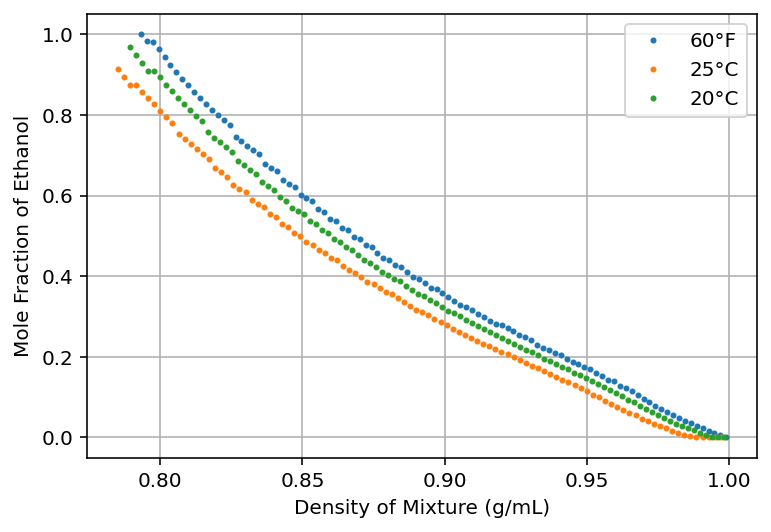
\includegraphics[width=3.6in]{fig1}
		\caption{Measured voltage readings from a PendoTec single-use pressure sensor recorded at various static pressures from a gas piston apparatus containing air. Static pressures were induced by adding weights of [84.248 $\pm$ 0.007g; 164.817 $\pm$ 0.007g; 239.434 $\pm$ 0.002g; 328.00 $\pm$ 0.01g and 402.531 $\pm$ 0.003g.] to the apparatus and appear in the figure from left to right. Error bars were calculated based on a 95\% confidence interval of recorded voltage readings in mV across three trials for each pressure (N=2). Uncertainty }
		\label{fig_1}
	\end{figure}
	\begin{table*}[!htbp]
		\centering
		\caption{Gas Properties}
		\label{tab:gas_properties}
		\begin{tabular}{lcccccc}
			\toprule
			Gas & Condition & $P_0$ (Pa) & $C$ (Pa) & $\kappa$ (s$^{-1}$) & $\omega$ (rad s$^{-1}$) & $\phi$ (rad) \\
			\midrule
			Air & Empty & $102171.80 \pm 7.20$ & $4518.24 \pm 886.00$ & $37.53 \pm 2.97$ & $217.85 \pm 2.87$ & $-9.62 \pm 3.02$ \\
			& 1 Weight & $103076.35 \pm 2.59$ & $2061.26 \pm 545.07$ & $14.59 \pm 1.03$ & $118.06 \pm 0.64$ & $-10.88 \pm 7.99$ \\
			& 2 Weight & $103389.06 \pm 1.81$ & $4264.83 \pm 513.42$ & $10.45 \pm 0.76$ & $90.98 \pm 0.63$ & $-8.53 \pm 6.94$ \\
			& 3 Weight & $104821.81 \pm 12.52$ & $-1212.16 \pm 513.84$ & $10.03 \pm 0.56$ & $79.06 \pm 0.73$ & $-15.93 \pm 9.20$ \\
			Argon & Empty & $102269.40 \pm 4.39$ & $-1487.97 \pm 3403.32$ & $16.59 \pm 4.37$ & $207.72 \pm 0.38$ & $-12.77 \pm 6.63$ \\
			& 1 Weight & $103093.24 \pm 3.53$ & $23.81 \pm 945.56$ & $15.69 \pm 0.08$ & $120.07 \pm 0.51$ & $-15.62 \pm 4.69$ \\
			& 2 Weight & $104000.11 \pm 21.84$ & $1201.48 \pm 2621.70$ & $17.28 \pm 1.22$ & $80.95 \pm 0.35$ & $-31.05 \pm 8.21$ \\
			& 3 Weight & $104882.66 \pm 36.64$ & $349.51 \pm 7984.72$ & $14.13 \pm 0.50$ & $77.39 \pm 0.91$ & $-15.90 \pm 11.16$ \\
			CO$_2$ & Empty & $102304.81 \pm 15.52$ & $882.70 \pm 1867.09$ & $32.71 \pm 5.98$ & $178.53 \pm 1.66$ & $-22.61 \pm 15.44$ \\
			& 1 Weight & $102216.12 \pm 3.98$ & $890.54 \pm 3907.62$ & $14.78 \pm 3.93$ & $106.12 \pm 2.15$ & $-22.41 \pm 23.91$ \\
			& 2 Weight & $103976.97 \pm 3.03$ & $-1087.62 \pm 2016.17$ & $9.09 \pm 1.17$ & $83.14 \pm 0.42$ & $-25.64 \pm 13.47$ \\
			& 3 Weight & $104000.26 \pm 14.20$ & $-6199.73 \pm 518.83$ & $6.59 \pm 1.27$ & $68.67 \pm 0.14$ & $-13.64 \pm 11.07$ \\
			\bottomrule
		\end{tabular}
	\end{table*}
	
	
	\begin{figure*}[!t]
		\centering
		\subfloat[]{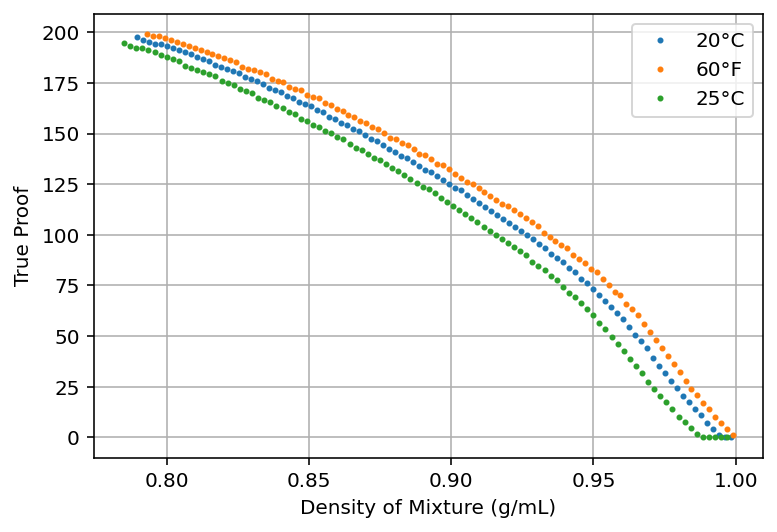
\includegraphics[width=5in]{fig2}%
			\label{a}}
		\hfil
		\caption{Dae. Ad quatur autat ut porepel itemoles dolor autem fuga. Bus quia con nessunti as remo di quatus non perum que nimus. (a) Case I. (b) Case II.}
		
	\end{figure*}
	
	Note that often IEEE papers with multi-part figures do not place the labels within the image itself (using the optional argument to $\backslash${\tt{subfloat}}[]), but instead will
	reference/describe all of them (a), (b), etc., within the main caption.
	Be aware that for subfig.sty to generate the (a), (b), etc., subfigure
	labels, the optional argument to $\backslash${\tt{subfloat}} must be present. If a
	subcaption is not desired, leave its contents blank,
	e.g.,$\backslash${\tt{subfloat}}[].
	
	
	
	
	\section{Discussion}
	Note that, for IEEE-style tables, the
	$\backslash${\tt{caption}} command should come BEFORE the table. Table captions use title case. Articles (a, an, the), coordinating conjunctions (and, but, for, or, nor), and most short prepositions are lowercase unless they are the first or last word. Table text will default to $\backslash${\tt{footnotesize}} as
	the IEEE normally uses this smaller font for tables.
	The $\backslash${\tt{label}} must come after $\backslash${\tt{caption}} as always.
	
	
	\begin{table*}[!htbp]
		\centering
		\caption{$\kappa$ Values for Air, Argon, and CO$_2$}
		\label{tab:kappa_values}
		\begin{tabular}{lcccc}
			\toprule
			Gas & $\kappa_\text{Empty}$ & $\kappa_\text{1 Weight}$ & $\kappa_\text{2 Weight}$ & $\kappa_\text{3 Weight}$ \\ 
			\midrule
			Air & $1.37 \pm 4 \times 10^{-21}$ & $0.95 \pm 3 \times 10^{-21}$ & $1.10 \pm 3 \times 10^{-21}$ & $1.20 \pm 3 \times 10^{-21}$ \\
			Argon & $1.74 \pm 3 \times 10^{-21}$ & $1.61 \pm 4 \times 10^{-21}$ & $1.53 \pm 2 \times 10^{-21}$ & $1.64 \pm 3 \times 10^{-21}$ \\
			CO$_2$ & $1.28 \pm 1 \times 10^{-21}$ & $1.36 \pm 4 \times 10^{-21}$ & $1.32 \pm 2 \times 10^{-21}$ & $1.28 \pm 2 \times 10^{-21}$ \\
			\bottomrule
		\end{tabular}
	\end{table*}
	
	\section{Technical Advances}
	
	Typographical conventions for mathematical formulas have been developed to {\bf provide uniformity and clarity of presentation across mathematical texts}. This enables the readers of those texts to both understand the author's ideas and to grasp new concepts quickly. While software such as \LaTeX \ and MathType\textsuperscript{\textregistered} can produce aesthetically pleasing math when used properly, it is also very easy to misuse the software, potentially resulting in incorrect math display.
	
	IEEE aims to provide authors with the proper guidance on mathematical typesetting style and assist them in writing the best possible article. As such, IEEE has assembled a set of examples of good and bad mathematical typesetting \cite{ref1,ref2,ref3,ref4,ref5}. 
	
	Further examples can be found at \url{http://journals.ieeeauthorcenter.ieee.org/wp-content/uploads/sites/7/IEEE-Math-Typesetting-Guide-for-LaTeX-Users.pdf}
	
	\subsection{Display Equations}
	The simple display equation example shown below uses the ``equation'' environment. To number the equations, use the $\backslash${\tt{label}} macro to create an identifier for the equation. LaTeX will automatically number the equation for you.
	\begin{equation}
		\label{deqn_ex1}
		x = \sum_{i=0}^{n} 2{i} Q.
	\end{equation}
	
	\noindent is coded as follows:
	\begin{verbatim}
		\begin{equation}
			\label{deqn_ex1}
			x = \sum_{i=0}^{n} 2{i} Q.
		\end{equation}
	\end{verbatim}
	
	To reference this equation in the text use the $\backslash${\tt{ref}} macro. 
	Please see (\ref{deqn_ex1})\\
	\noindent is coded as follows:
	\begin{verbatim}
		Please see (\ref{deqn_ex1})\end{verbatim}
	
	\subsection{Equation Numbering}
	{\bf{Consecutive Numbering:}} Equations within an article are numbered consecutively from the beginning of the
	article to the end, i.e., (1), (2), (3), (4), (5), etc. Do not use roman numerals or section numbers for equation numbering.
	
	\noindent {\bf{Appendix Equations:}} The continuation of consecutively numbered equations is best in the Appendix, but numbering
	as (A1), (A2), etc., is permissible.\\
	
	\noindent {\bf{Hyphens and Periods}}: Hyphens and periods should not be used in equation numbers, i.e., use (1a) rather than
	(1-a) and (2a) rather than (2.a) for subequations. This should be consistent throughout the article.
	
	\subsection{Multi-Line Equations and Alignment}
	Here we show several examples of multi-line equations and proper alignments.
	
	\noindent {\bf{A single equation that must break over multiple lines due to length with no specific alignment.}}
	\begin{multline}
		\text{The first line of this example}\\
		\text{The second line of this example}\\
		\text{The third line of this example}
	\end{multline}
	
	\noindent is coded as:
	\begin{verbatim}
		\begin{multline}
			\text{The first line of this example}\\
			\text{The second line of this example}\\
			\text{The third line of this example}
		\end{multline}
	\end{verbatim}
	
	\noindent {\bf{A single equation with multiple lines aligned at the = signs}}
	\begin{align}
		a &= c+d \\
		b &= e+f
	\end{align}
	\noindent is coded as:
	\begin{verbatim}
		\begin{align}
			a &= c+d \\
			b &= e+f
		\end{align}
	\end{verbatim}
	
	The {\tt{align}} environment can align on multiple  points as shown in the following example:
	\begin{align}
		x &= y & X & =Y & a &=bc\\
		x' &= y' & X' &=Y' &a' &=bz
	\end{align}
	\noindent is coded as:
	\begin{verbatim}
		\begin{align}
			x &= y & X & =Y & a &=bc\\
			x' &= y' & X' &=Y' &a' &=bz
		\end{align}
	\end{verbatim}
	
	
	
	
	
	\subsection{Subnumbering}
	The amsmath package provides a {\tt{subequations}} environment to facilitate subnumbering. An example:
	
	\begin{subequations}\label{eq:2}
		\begin{align}
			f&=g \label{eq:2A}\\
			f' &=g' \label{eq:2B}\\
			\mathcal{L}f &= \mathcal{L}g \label{eq:2c}
		\end{align}
	\end{subequations}
	
	\noindent is coded as:
	\begin{verbatim}
		\begin{subequations}\label{eq:2}
			\begin{align}
				f&=g \label{eq:2A}\\
				f' &=g' \label{eq:2B}\\
				\mathcal{L}f &= \mathcal{L}g \label{eq:2c}
			\end{align}
		\end{subequations}
		
	\end{verbatim}
	
	\subsection{Matrices}
	There are several useful matrix environments that can save you some keystrokes. See the example coding below and the output.
	
	\noindent {\bf{A simple matrix:}}
	\begin{equation}
		\begin{matrix}  0 &  1 \\ 
			1 &  0 \end{matrix}
	\end{equation}
	is coded as:
	\begin{verbatim}
		\begin{equation}
			\begin{matrix}  0 &  1 \\ 
				1 &  0 \end{matrix}
		\end{equation}
	\end{verbatim}
	
	\noindent {\bf{A matrix with parenthesis}}
	\begin{equation}
		\begin{pmatrix} 0 & -i \\
			i &  0 \end{pmatrix}
	\end{equation}
	is coded as:
	\begin{verbatim}
		\begin{equation}
			\begin{pmatrix} 0 & -i \\
				i &  0 \end{pmatrix}
		\end{equation}
	\end{verbatim}
	
	\noindent {\bf{A matrix with square brackets}}
	\begin{equation}
		\begin{bmatrix} 0 & -1 \\ 
			1 &  0 \end{bmatrix}
	\end{equation}
	is coded as:
	\begin{verbatim}
		\begin{equation}
			\begin{bmatrix} 0 & -1 \\ 
				1 &  0 \end{bmatrix}
		\end{equation}
	\end{verbatim}
	
	\noindent {\bf{A matrix with curly braces}}
	\begin{equation}
		\begin{Bmatrix} 1 &  0 \\ 
			0 & -1 \end{Bmatrix}
	\end{equation}
	is coded as:
	\begin{verbatim}
		\begin{equation}
			\begin{Bmatrix} 1 &  0 \\ 
				0 & -1 \end{Bmatrix}
	\end{equation}\end{verbatim}
	
	\noindent {\bf{A matrix with single verticals}}
	\begin{equation}
		\begin{vmatrix} a &  b \\ 
			c &  d \end{vmatrix}
	\end{equation}
	is coded as:
	\begin{verbatim}
		\begin{equation}
			\begin{vmatrix} a &  b \\ 
				c &  d \end{vmatrix}
	\end{equation}\end{verbatim}
	
	\noindent {\bf{A matrix with double verticals}}
	\begin{equation}
		\begin{Vmatrix} i &  0 \\ 
			0 & -i \end{Vmatrix}
	\end{equation}
	is coded as:
	\begin{verbatim}
		\begin{equation}
			\begin{Vmatrix} i &  0 \\ 
				0 & -i \end{Vmatrix}
	\end{equation}\end{verbatim}
	
	\subsection{Arrays}
	The {\tt{array}} environment allows you some options for matrix-like equations. You will have to manually key the fences, but there are other options for alignment of the columns and for setting horizontal and vertical rules. The argument to {\tt{array}} controls alignment and placement of vertical rules.
	
	A simple array
	\begin{equation}
		\left(
		\begin{array}{cccc}
			a+b+c & uv & x-y & 27\\
			a+b & u+v & z & 134
		\end{array}\right)
	\end{equation}
	is coded as:
	\begin{verbatim}
		\begin{equation}
			\left(
			\begin{array}{cccc}
				a+b+c & uv & x-y & 27\\
				a+b & u+v & z & 134
			\end{array} \right)
		\end{equation}
	\end{verbatim}
	
	A slight variation on this to better align the numbers in the last column
	\begin{equation}
		\left(
		\begin{array}{cccr}
			a+b+c & uv & x-y & 27\\
			a+b & u+v & z & 134
		\end{array}\right)
	\end{equation}
	is coded as:
	\begin{verbatim}
		\begin{equation}
			\left(
			\begin{array}{cccr}
				a+b+c & uv & x-y & 27\\
				a+b & u+v & z & 134
			\end{array} \right)
		\end{equation}
	\end{verbatim}
	
	An array with vertical and horizontal rules
	\begin{equation}
		\left( \begin{array}{c|c|c|r}
			a+b+c & uv & x-y & 27\\ \hline
			a+b & u+v & z & 134
		\end{array}\right)
	\end{equation}
	is coded as:
	\begin{verbatim}
		\begin{equation}
			\left(
			\begin{array}{c|c|c|r}
				a+b+c & uv & x-y & 27\\
				a+b & u+v & z & 134
			\end{array} \right)
		\end{equation}
	\end{verbatim}
	Note the argument now has the pipe "$\vert$" included to indicate the placement of the vertical rules.
	
	
	\subsection{Cases Structures}
	Many times cases can be miscoded using the wrong environment, i.e., {\tt{array}}. Using the {\tt{cases}} environment will save keystrokes (from not having to type the $\backslash${\tt{left}}$\backslash${\tt{lbrace}}) and automatically provide the correct column alignment.
	\begin{equation*}
		{z_m(t)} = \begin{cases}
			1,&{\text{if}}\ {\beta }_m(t) \\ 
			{0,}&{\text{otherwise.}} 
		\end{cases}
	\end{equation*}
	\noindent is coded as follows:
	\begin{verbatim}
		\begin{equation*}
			{z_m(t)} = 
			\begin{cases}
				1,&{\text{if}}\ {\beta }_m(t),\\ 
				{0,}&{\text{otherwise.}} 
			\end{cases}
		\end{equation*}
	\end{verbatim}
	\noindent Note that the ``\&'' is used to mark the tabular alignment. This is important to get  proper column alignment. Do not use $\backslash${\tt{quad}} or other fixed spaces to try and align the columns. Also, note the use of the $\backslash${\tt{text}} macro for text elements such as ``if'' and ``otherwise.''
	
	\subsection{Function Formatting in Equations}
	Often, there is an easy way to properly format most common functions. Use of the $\backslash$ in front of the function name will in most cases, provide the correct formatting. When this does not work, the following example provides a solution using the $\backslash${\tt{text}} macro:
	
	\begin{equation*} 
		d_{R}^{KM} = \underset {d_{l}^{KM}} {\text{arg min}} \{ d_{1}^{KM},\ldots,d_{6}^{KM}\}.
	\end{equation*}
	
	\noindent is coded as follows:
	\begin{verbatim}
		\begin{equation*} 
			d_{R}^{KM} = \underset {d_{l}^{KM}} 
			{\text{arg min}} \{ d_{1}^{KM},
			\ldots,d_{6}^{KM}\}.
		\end{equation*}
	\end{verbatim}
	
	\subsection{ Text Acronyms Inside Equations}
	This example shows where the acronym ``MSE" is coded using $\backslash${\tt{text\{\}}} to match how it appears in the text.
	
	\begin{equation*}
		\text{MSE} = \frac {1}{n}\sum _{i=1}^{n}(Y_{i} - \hat {Y_{i}})^{2}
	\end{equation*}
	
	\begin{verbatim}
		\begin{equation*}
			\text{MSE} = \frac {1}{n}\sum _{i=1}^{n}
			(Y_{i} - \hat {Y_{i}})^{2}
		\end{equation*}
	\end{verbatim}
	
	\section{Conclusion}
	The conclusion goes here.
	
	
	
	
	
	{\appendix[Proof of the Zonklar Equations]
		Use $\backslash${\tt{appendix}} if you have a single appendix:
		Do not use $\backslash${\tt{section}} anymore after $\backslash${\tt{appendix}}, only $\backslash${\tt{section*}}.
		If you have multiple appendixes use $\backslash${\tt{appendices}} then use $\backslash${\tt{section}} to start each appendix.
		You must declare a $\backslash${\tt{section}} before using any $\backslash${\tt{subsection}} or using $\backslash${\tt{label}} ($\backslash${\tt{appendices}} by itself
		starts a section numbered zero.)}
	
	
	
	%{\appendices
		%\section*{Proof of the First Zonklar Equation}
		%Appendix one text goes here.
		% You can choose not to have a title for an appendix if you want by leaving the argument blank
		%\section*{Proof of the Second Zonklar Equation}
		%Appendix two text goes here.}
	
	
	
	\section{References Section}
	You can use a bibliography generated by BibTeX as a .bbl file.
	BibTeX documentation can be easily obtained at:
	http://mirror.ctan.org/biblio/bibtex/contrib/doc/
	The IEEEtran BibTeX style support page is:
	http://www.michaelshell.org/tex/ieeetran/bibtex/
	
	% argument is your BibTeX string definitions and bibliography database(s)
	%\bibliography{IEEEabrv,../bib/paper}
	%
	\section{Simple References}
	You can manually copy in the resultant .bbl file and set second argument of $\backslash${\tt{begin}} to the number of references
	(used to reserve space for the reference number labels box).
	
	\begin{thebibliography}{1}
		\bibliographystyle{IEEEtran}
		
		\bibitem{ref1}
		{\it{Mathematics Into Type}}. American Mathematical Society. [Online]. Available: https://www.ams.org/arc/styleguide/mit-2.pdf
		
		\bibitem{ref2}
		T. W. Chaundy, P. R. Barrett and C. Batey, {\it{The Printing of Mathematics}}. London, U.K., Oxford Univ. Press, 1954.
		
		\bibitem{ref3}
		F. Mittelbach and M. Goossens, {\it{The \LaTeX Companion}}, 2nd ed. Boston, MA, USA: Pearson, 2004.
		
		\bibitem{ref4}
		G. Gr\"atzer, {\it{More Math Into LaTeX}}, New York, NY, USA: Springer, 2007.
		
		\bibitem{ref5}M. Letourneau and J. W. Sharp, {\it{AMS-StyleGuide-online.pdf,}} American Mathematical Society, Providence, RI, USA, [Online]. Available: http://www.ams.org/arc/styleguide/index.html
		
		\bibitem{ref6}
		H. Sira-Ramirez, ``On the sliding mode control of nonlinear systems,'' \textit{Syst. Control Lett.}, vol. 19, pp. 303--312, 1992.
		
		\bibitem{ref7}
		A. Levant, ``Exact differentiation of signals with unbounded higher derivatives,''  in \textit{Proc. 45th IEEE Conf. Decis.
			Control}, San Diego, CA, USA, 2006, pp. 5585--5590. DOI: 10.1109/CDC.2006.377165.
		
		\bibitem{ref8}
		M. Fliess, C. Join, and H. Sira-Ramirez, ``Non-linear estimation is easy,'' \textit{Int. J. Model., Ident. Control}, vol. 4, no. 1, pp. 12--27, 2008.
		
		\bibitem{ref9}
		R. Ortega, A. Astolfi, G. Bastin, and H. Rodriguez, ``Stabilization of food-chain systems using a port-controlled Hamiltonian description,'' in \textit{Proc. Amer. Control Conf.}, Chicago, IL, USA,
		2000, pp. 2245--2249.
		
	\end{thebibliography}
	
	
	\newpage
	
	\section{Biography Section}
	If you have an EPS/PDF photo (graphicx package needed), extra braces are
	needed around the contents of the optional argument to biography to prevent
	the LaTeX parser from getting confused when it sees the complicated
	$\backslash${\tt{includegraphics}} command within an optional argument. (You can create
	your own custom macro containing the $\backslash${\tt{includegraphics}} command to make things
	simpler here.)
	
	\vspace{11pt}
	
	\bf{If you include a photo:}\vspace{-33pt}
	\begin{IEEEbiography}[{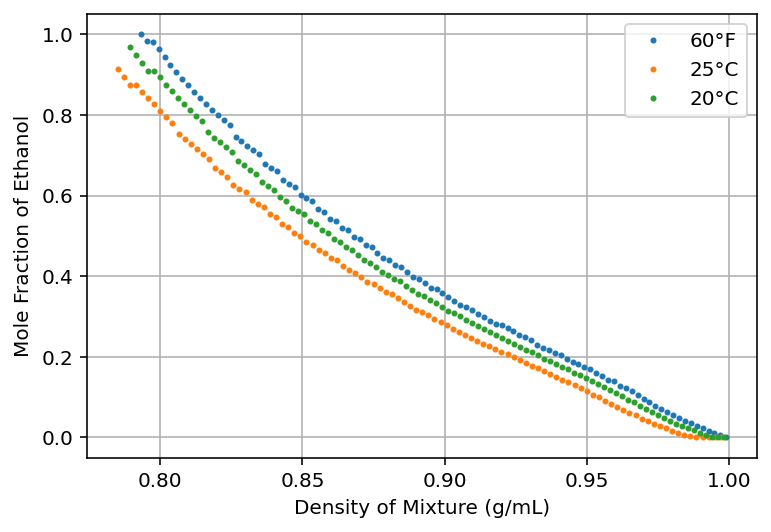
\includegraphics[width=1in,height=1.25in,clip,keepaspectratio]{fig1}}]{Michael Shell}
		Use $\backslash${\tt{begin\{IEEEbiography\}}} and then for the 1st argument use $\backslash${\tt{includegraphics}} to declare and link the author photo.
		Use the author name as the 3rd argument followed by the biography text.
	\end{IEEEbiography}
	
	\vspace{11pt}
	
	\bf{If you will not include a photo:}\vspace{-33pt}
	\begin{IEEEbiographynophoto}{John Doe}
		Use $\backslash${\tt{begin\{IEEEbiographynophoto\}}} and the author name as the argument followed by the biography text.
	\end{IEEEbiographynophoto}
	
	
	
	
	\vfill
	
\end{document}


